\documentclass[11pt]{article}
\usepackage[margin=1in]{geometry}
\usepackage{amsmath,amssymb,amsfonts}
\usepackage{graphicx,float}
\usepackage{fancyhdr,booktabs}
\usepackage{listings}
\usepackage{hyperref}
\usepackage{listings, soul}
\usepackage[most]{tcolorbox}
\tcbset{breakable}
\usepackage{tikz}
\usetikzlibrary{arrows.meta, positioning, calc}

\lstset{
    language=Matlab,
    basicstyle=\ttfamily\small,
    breaklines=true,
    keepspaces=true,
    showstringspaces=false
}


\title{\textbf{ME 352 Workshop}\\[0.5ex]\Large In-class Freq Response Workshop}
\author{Zeshui Song}
\date{Fall 2026}

\begin{document}
\maketitle
\vspace{-1em}

\section*{Frequency Response Design of a Controller}

\begin{center}
    
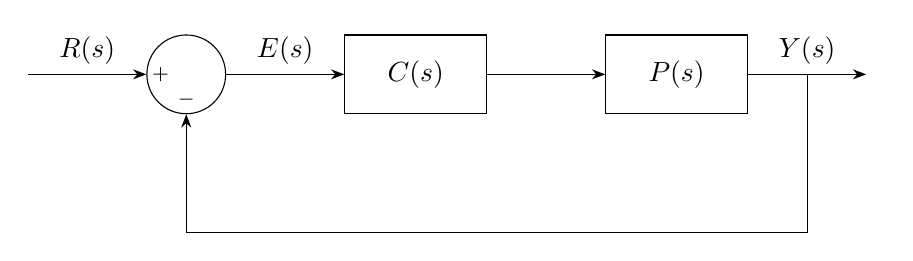
\begin{tikzpicture}[
    >=Stealth,
    block/.style={
        draw, rectangle,
        minimum width=1.8cm,
        minimum height=1cm
    },
    sum/.style={
        draw, circle,
        minimum size=1cm,
        inner sep=0pt
    },
    node distance=1.5cm
]

    % Nodes
    \node[sum] (sum) {};
    \node[block, right=1.5cm of sum] (controller) {$C(s)$};
    \node[block, right=1.5cm of controller] (plant) {$P(s)$};
    \node[right=1.5cm of plant] (output) {};

    % Forward path
    \draw[->] ([xshift=-1.5cm]sum.west)
        -- node[above] {$R(s)$} (sum.west);

    \draw[->] (sum.east)
        -- node[above] {$E(s)$} (controller.west);

    \draw[->] (controller.east) -- (plant.west);

    \draw[->] (plant.east)
        -- node[above] {$Y(s)$} (output);

    % Unity negative feedback
    \draw[->] ($(plant.east)+(0.75cm,0)$)
        |- ($(sum.south)+(0,-1.5cm)$)
        -- (sum.south);

    % Summing junction signs
    \node at ($(sum.west)+(0.18cm,0)$) {\scriptsize $+$};
    \node at ($(sum.south)+(0,0.18cm)$) {\scriptsize $-$};

\end{tikzpicture}
\end{center}
Previously, we modeled the DC motor as a first order system with transfer function
\[
\frac{\Omega(s)}{U(s)}=\frac{1}{\tau s+1}
\]
Here, we will design a position controller for the DC motor using frequency response methods. We obtain the position transfer function by multiplying the velocity transfer function by an integrator:
\[
P(s)=\frac{\Theta(s)}{U(s)}=\frac{1}{s(\tau s+1)}
\]
With a proportional controller, the loop transfer function is
\[
L(s)=C(s)P(s)=\frac{K}{s(\tau s+1)}
\]
\subsection*{Bode plot}
For $K=1$, $\tau=1$, the Bode plot is as follows:
\begin{itemize}
    \item We start at the DC gain of the system. However, because the system has an integrator, the DC gain is infinite. Therefore, we approximate the start point by considering the magnitude at a low frequency, say $\omega=0.1$ rad/s:
    \[L(\hat{\imath}) \approx \frac{1}{\hat{\imath} \omega}\quad \implies \quad |L(\hat{\imath}\omega)| \approx \frac{1}{\omega}\]
    Converting to dB, we have
    \[20\log_{10}|L(\hat{\imath}\omega)| \approx 20\log_{10}\left(\frac{1}{\omega}\right) = -20\log_{10}(\omega)\]
    At $\omega=0.01$ rad/s,
    \[|L(0.01\hat{\imath})| \approx 40\]
    Note that as we approach $\omega=0$, the magnitude approaches infinity, but for sketching, we can start at a finite value close to the origin (e.g., 40 dB at $\omega=0.01$ rad/s).
    \item Finding the corner frequencies:
    \begin{itemize}
        \item The integrator gives a slope of $-20$ dB/decade starting from $\omega=0.01$ rad/s.
        \item The pole at $s=-1$ gives a corner frequency at $\omega=1$ rad/s, where the slope changes from $-20$ dB/decade to $-40$ dB/decade.
        \item The phase starts at $-90^\circ$ due to the integrator and the pole at $s=-1$ contributes an additional $-90^\circ$ phase lag, resulting in a total phase of $-180^\circ$ at the corner frequency $\omega=1$ rad/s.
    \end{itemize}
    \begin{center}
    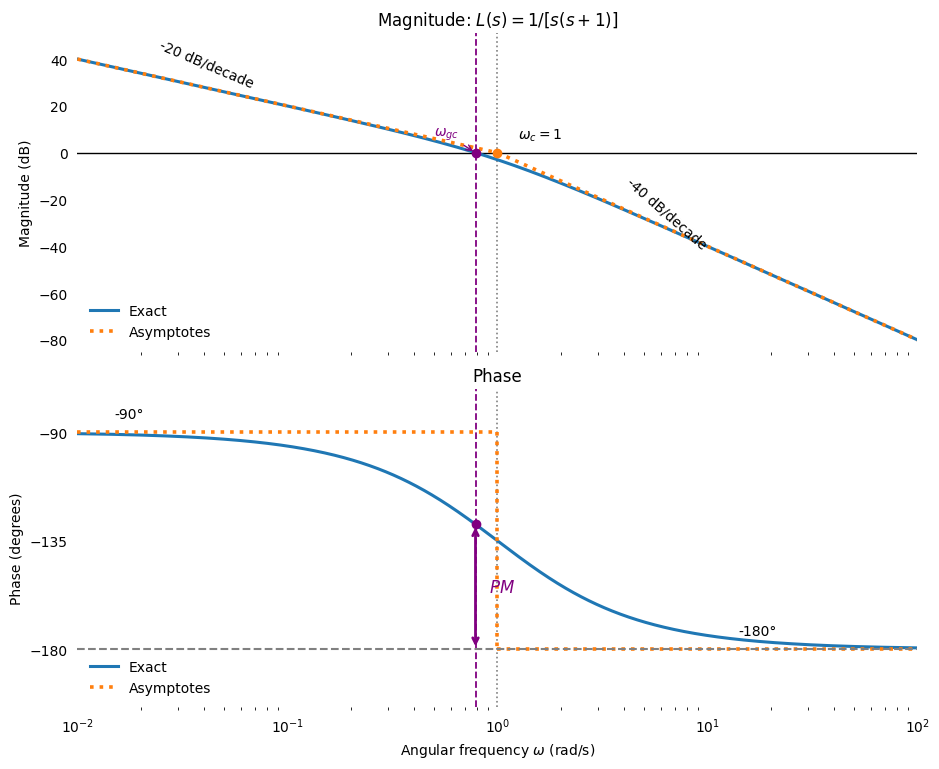
\includegraphics[width=0.8\textwidth]{position bode.png}
\end{center}
    \begin{tcolorbox}
    Note: for a general transfer function of the form
    \[G(s) = \frac{a}{s+a}\]
    With a pole at $s=-a$ ($a>0$), we can find the corner frequencies by considering the asymptotic behavior of the phase and magnitude plots.
    \begin{itemize}
        \item For $\omega \ll a$:
        \[|G(\hat{\imath}\omega)| \approx \frac{a}{a} = 1\quad \implies \quad 20\log_{10}|G(\hat{\imath}\omega)| \approx 0\, dB\]
        \[\angle G(\hat{\imath}\omega) \approx \angle 1 = 0^\circ\]
        \item For $\omega \gg a$:
        \[|G(\hat{\imath}\omega)| \approx \frac{a}{\hat{\imath}\omega} = \frac{a}{\omega} \quad \implies \quad 20\log_{10}|G(\hat{\imath}\omega)| \approx 20\log_{10}(a) - 20\log_{10}(\omega)\,dB\]
        \[\angle G(\hat{\imath}\omega) \approx \angle \frac{a}{\hat{\imath}\omega} = \angle a - \angle \hat{\imath}\omega = -90^\circ\]
        Note that for a logarithmic scale for $\omega$, the asymptote for the magnitude plot is a straight line with slope $-20$ dB/decade!
    \end{itemize}
    Therefore, the corner frequency is at $\omega_c=a$, where the asymptotes intersect:
    \[0 = 20\log_{10}(a) - 20\log_{10}(\omega_c) \quad \implies \quad \omega_c = a\]
    \begin{center}
        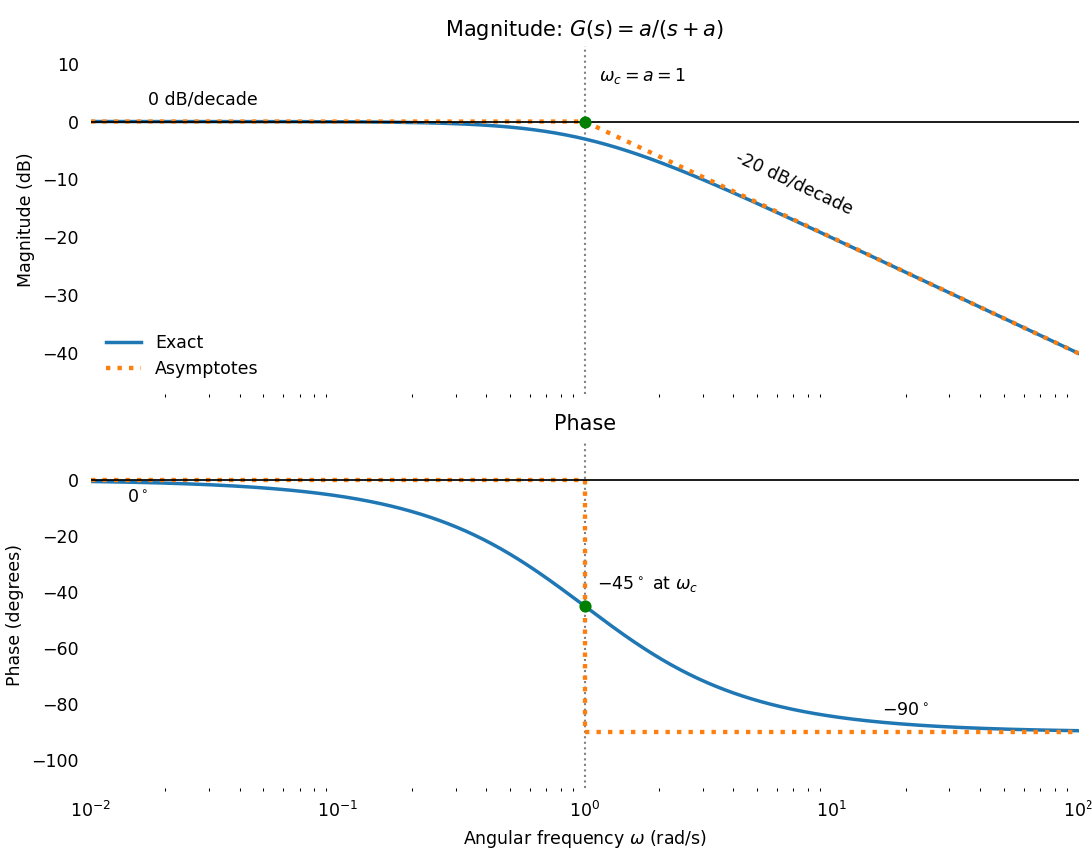
\includegraphics[width=0.8\textwidth]{ex bode.png}
    \end{center}
    \end{tcolorbox}
\end{itemize}
\underline{Note:} The gain crossover frequency $\omega_{gc}$ is the frequency at which the magnitude of the loop transfer function is 0 dB. This is NOT equal to the corner frequency!
\subsection*{Phase Margin}
Recall that the gain crossover frequency $\omega_{gc}$ is defined by
\[|L(\hat{\imath}\omega_{gc})| = 1 = 0\, \text{dB}\]
The phase margin is defined as the additional phase lag required to reach $-180^\circ$ at the gain crossover frequency:
\[\text{PM} = 180^\circ + \angle L(\hat{\imath}\omega_{gc})\]
\begin{tcolorbox}
Recall that the closed-loop transfer function is given by
\[
T(s)=\frac{L(s)}{1+L(s)}
\]
with poles determined by the roots of the characteristic equation
\[
1+L(s)=0
\]
For the closed-loop system to have poles on the imaginary axis, we require
\[
1+L(\hat{\imath}\omega)=0
\quad \implies \quad
L(\hat{\imath}\omega)=-1
\]
Equivalently, this gives the magnitude and phase conditions
\[
|L(\hat{\imath}\omega)|=1
\qquad \text{and} \qquad
\angle L(\hat{\imath}\omega)=-180^\circ
\]
\hl{The frequencies at which both conditions are satisfied correspond to closed-loop poles at $s=\pm\hat{\imath}\omega$, indicating the boundary of stability, where the system exhibits purely oscillatory behavior. }
\end{tcolorbox}
\noindent
\textbf{Phase Margin is related to damping ratio}\\
The standard second-order system transfer function has form:
\[
T(s)=\frac{\omega_n^2}{s^2+2\zeta\omega_n s+\omega_n^2}
\]
For unity negative feedback, the corresponding loop transfer function has form:
\[
L(s)=\frac{\omega_n^2}{s(s+2\zeta\omega_n)}
\]
Thus we can derive that:
\[
\boxed{PM=\tan^{-1}\left(\frac{2\zeta\omega_n}{\omega_{gc}}\right)=\tan^{-1}\left(\frac{2\zeta}{\sqrt{\sqrt{1+4\zeta^4}-2\zeta^2}}\right)}
\]
Or approximately, for small $\zeta$:
\[\boxed{\zeta \approx \frac{\text{PM}}{100}, \quad \text{(where PM is in degrees)}}\]
\section*{Lead/Lag Compensation}
Lead and lag compensators modify the loop transfer function by introducing an additional pole and zero, with the goal of shaping the Bode magnitude and phase plots to improve closed-loop performance (loop shaping).\\\\
The general form is:
\[C(s) = K_c\frac{s+z}{s+p}\]
Where $z$ is the zero, $p$ is the pole, and $K_c$ is the controller gain.
\subsection*{Lead Compensator} 
A lead compensator has a zero that is closer to the origin than its pole \hl{($|z|<|p|$)}. \\\\
The maximum phase lead occurs at $\omega_m = \sqrt{zp}$.\\\\
The purpose of a lead compensator is to add positive phase \textit{near the gain crossover frequency}, to increase the phase margin.
\subsection*{Lag Compensator}
For a lag compensator, the pole is closer to the origin than the zero \hl{($|p|<|z|$)}.\\\\
The purpose of a lag compensator is to improve steady-state tracking by increasing the low-frequency gain of the loop transfer function, while having minimal effect on the phase margin (add the lag compensator far away from the gain crossover frequency).
\begin{center}
    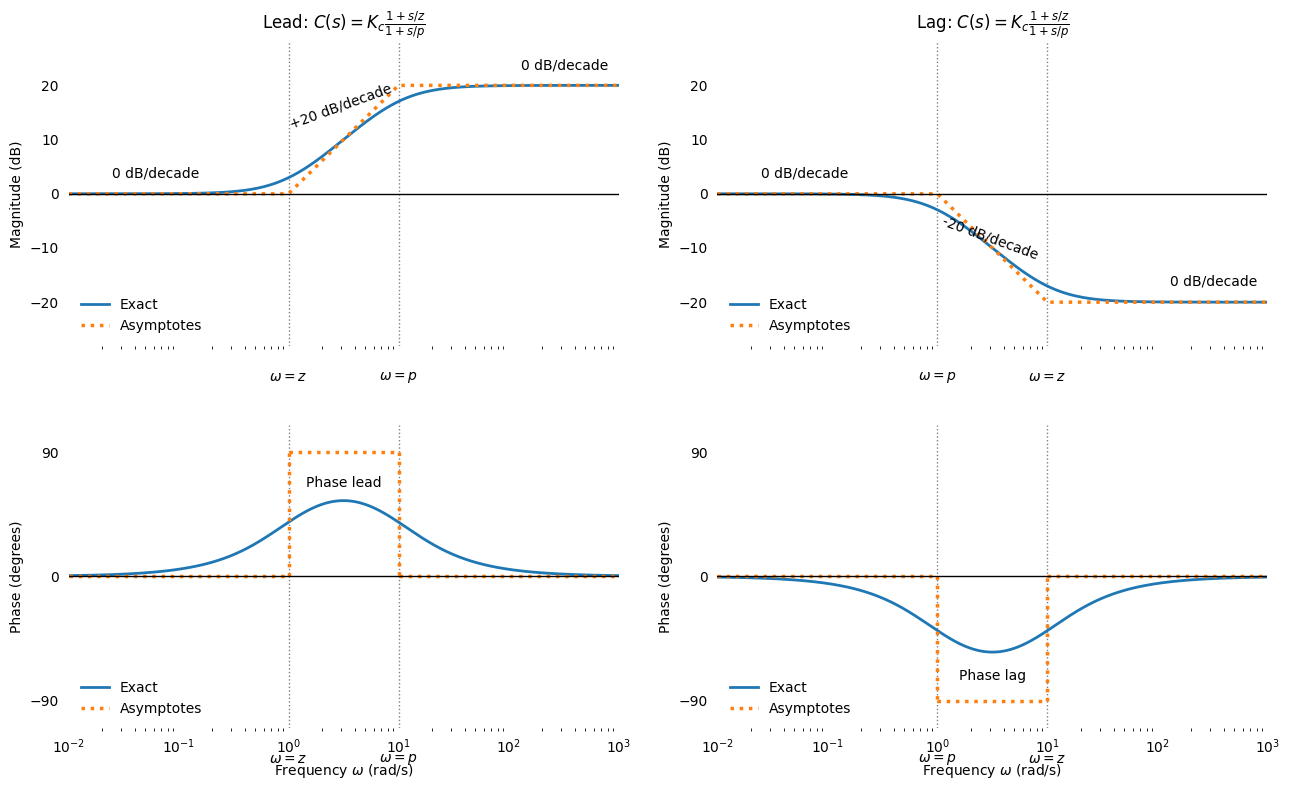
\includegraphics[width=\textwidth]{lead lag comp.png}
\end{center}
\hl{Make sure that the lag poles and zeros are not too close to the gain crossover frequency, otherwise they will reduce the phase margin!!}\\\\
\underline{Note:} Increasing the gain $K_c$ of the controller will move the gain crossover frequency! Since it will shift the magnitude plot up.\\
\noindent\rule{\textwidth}{0.5pt}
\newpage
\section*{Workshop}
Consider the plant transfer function
\[P(s) = \frac{1}{s(s+1)}\]
\subsection*{Problem 1:} Plot the uncompensated Bode Plot and determine the phase margin and crossover frequency.
\begin{center}
    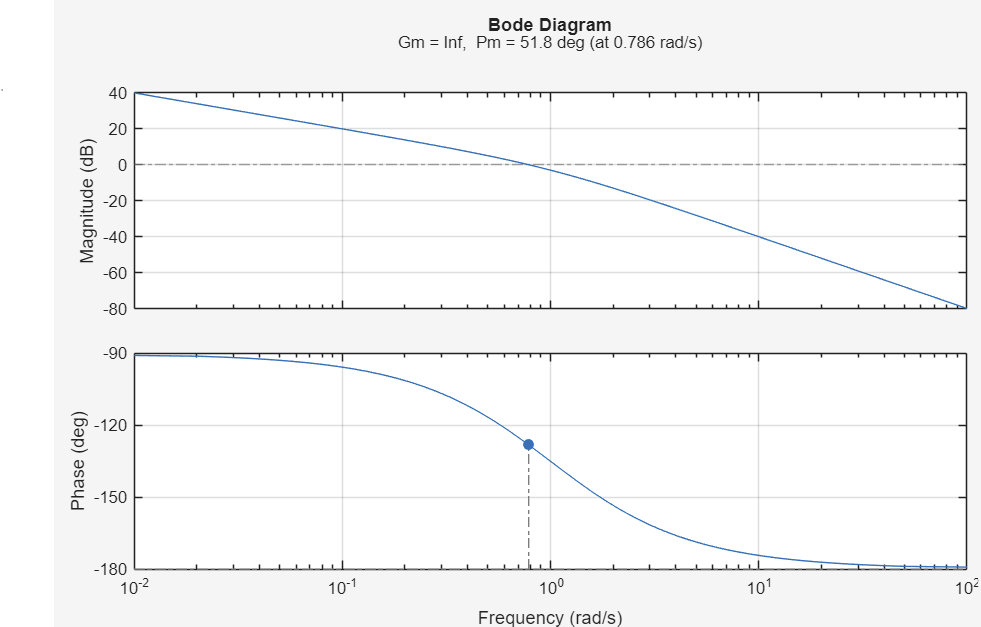
\includegraphics[width=0.7\textwidth]{P1.png}
\end{center}
PM = 51.8 deg, $\omega_{gc} = 0.786$ rad/s
\subsection*{Problem 2:} For the closed-loop case with P-Control where Kp=1, what is the steady-state error ($e_{ss}$) to step type inputs.
\[L(s)=C(s)P(s) = \frac{K_p}{s(s+1)},\quad K_p=1\]
\[\frac{E}{R} = \frac{1}{1+L(s)}\]
\[e_{ss}= \lim_{s \to 0} sE(s) = \lim_{s \to 0} s \cdot \frac{1}{s}\cdot\frac{1}{1+L(s)}=\lim_{s \to 0}\frac{s(s+1)}{s(s+1)+1}=0\]
\subsection*{Problem 3:} Add a lead controller of the form $C(s)=K_c(s+2)/(s+10)$.  By how much can you raise $K_c$ such that your PM$\geq$ 50 degrees. (Round up to the nearest integer)
\[L(s)=C(s)P(s) = \frac{K_c(s+2)}{s(s+1)(s+10)}\]
Use MATLAB to iteratively solve for the PM for each value of $K_c$ between 60 and 80 until for the value that satisfies the equation:
\[PM(K_c) = 50\]
for the maximum value of $K_c$ before the phase margin drops below 50 degrees.\\\\
It does this by finding the roots of the equation:
\[PM(K_c) - 50 = 0\]
In MATLAB:
\begin{lstlisting}
f = @(Kc) phaseMargin(Kc*C*P) - 50;
Kc = fzero(f, [60, 80]);
\end{lstlisting}
\begin{center}
    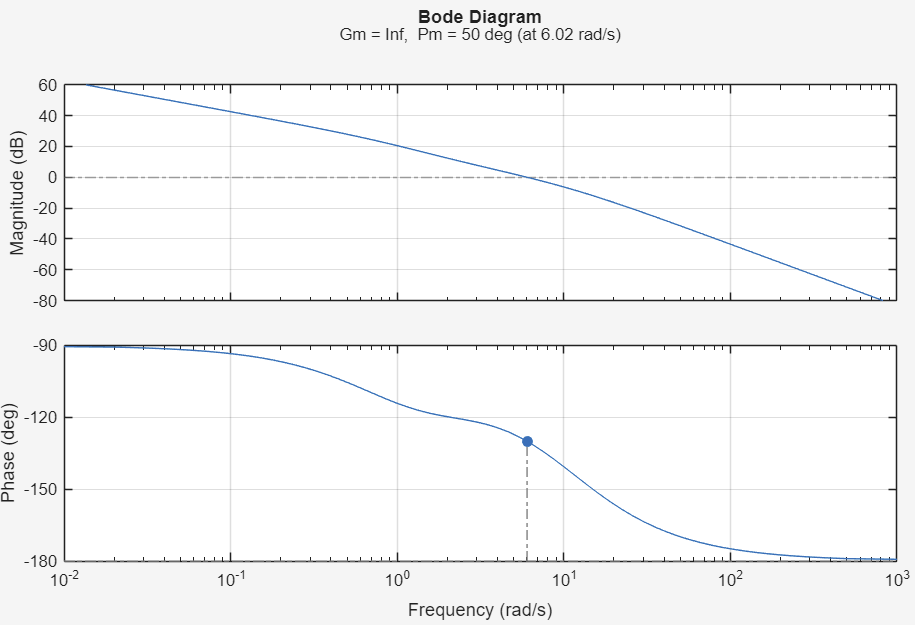
\includegraphics[width=0.7\textwidth]{P3.png}
\end{center}
Results: $K_c = 67.6265$ (round up to 68)\\\\
Increasing \(K_c\) shifts the magnitude Bode plot upward without changing the phase plot. Consequently, the gain crossover frequency increases, resulting in a smaller phase margin.
\subsection*{Problem 4:} For $K_c$ = 68, $z$=2, $p$=10, what is the steady-state error to a unit ramp input?
\[L(s)=C(s)P(s) = \frac{68(s+2)}{s(s+1)(s+10)}\]
\[
\begin{aligned}
e_{ss}
&= \lim_{s\to 0}sE(s)\\
&= \lim_{s\to 0}s\cdot\frac{1}{s^2}\cdot\frac{1}{1+L(s)}\\
&= \lim_{s\to 0}\frac{1}{s}\cdot\frac{s(s+1)(s+10)}{s(s+1)(s+10)+68(s+2)}\\
&= \lim_{s\to 0}\frac{(s+1)(s+10)}{s(s+1)(s+10)+68(s+2)}\\
&= \frac{10}{136}=\boxed{\frac{5}{68}\approx 0.0735}.
\end{aligned}
\]
\subsection*{Problem 5:} Add a lag compensator to try to reduce the error to a unit ramp less than or equal to 0.01.  What should the ratio $z/p$ be for the lag compensator?\\\\
With a lag compensator, the loop transfer function becomes:
\[L(s) = C(s)P(s) = \frac{68(s+2)}{s(s+1)(s+10)} \cdot \frac{(s-z)}{(s-p)},\quad p<z\]
\[
\begin{aligned}
e_{ss}
&= \lim_{s\to 0}sE(s)\\
&= \lim_{s\to 0}s\cdot\frac{1}{s^2}\cdot\frac{1}{1+L(s)}\\
&= \lim_{s\to 0}\frac{1}{s}\cdot
\frac{s(s+1)(s+10)(s-p)}
{s(s+1)(s+10)(s-p)+68(s+2)(s-z)}\\
&= \lim_{s\to 0}
\frac{(s+1)(s+10)(s-p)}
{s(s+1)(s+10)(s-p)+68(s+2)(s-z)}\\
&= \frac{-10p}{-136z}\\
&= \frac{5p}{68z}
\end{aligned}
\]
\[\frac{5p}{68z} \leq 0.01 \quad \implies \boxed{\frac{z}{p} \geq 7.3529}\]
\subsection*{Problem 6:} Compare the closed-loop step response for the proportional control case with $K_p=1$ with the closed-loop system with lead and lag compensation. Briefly describe the change in performance and briefly see if you can change the compensation to improve the response further. Briefly describe your final selection in gain and lead/lag zero and pole locations and any further improvements in response time, relative stability, etc.
\begin{center}
    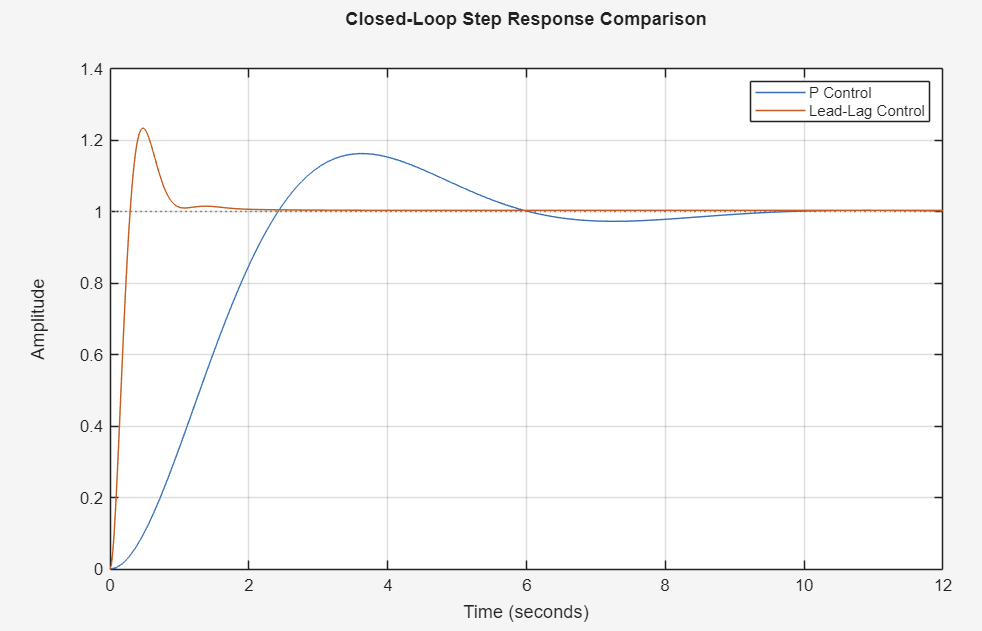
\includegraphics[width=0.7\textwidth]{P6.png}
\end{center}
I choose the lead compensator with $K_c=68$, $z=2$, $p=10$ to guarantee a phase margin of 50 degrees while increasing the speed of the system response by increasing the loop gain. Then, I added a lag compensator with a ratio of $z/p=7.3529$ to reduce the steady-state error to a unit ramp input to less than or equal to 0.01. In order for the lag compensator to have minimal effect on the phase margin, I placed the lag pole and zero close to the origin and far away from the gain crossover frequency (and the lead compensator zero and pole). This compensated system has a much faster rise and settling time than proportional control alone, however the overshoot is slightly larger. 
\subsection*{Problem 7:} Consider the new plant transfer function
\[P(s) = \frac{10}{(s+1)(s+4)}\]
 find the low frequency gain (DC Gain) of the uncompensated transfer function.
 \[
\begin{aligned}
y_{ss}
&= \lim_{s\to 0}sY(s)\\
&= \lim_{s\to 0}s\cdot\frac{10}{(s+1)(s+4)}\cdot\frac{1}{s}\\
&= \lim_{s\to 0}\frac{10}{(s+1)(s+4)}\\
&= \boxed{\frac{10}{4}=2.5}.
\end{aligned}
\]
\subsection*{Problem 8.} Add compensation to improve the closed loop behavior (both transient and steady-state response).  Describe your process, the compensation selected and how you improved the response compared to the uncompensated system.\\\\
\underline{Understand the uncompensated system}
\begin{center}
    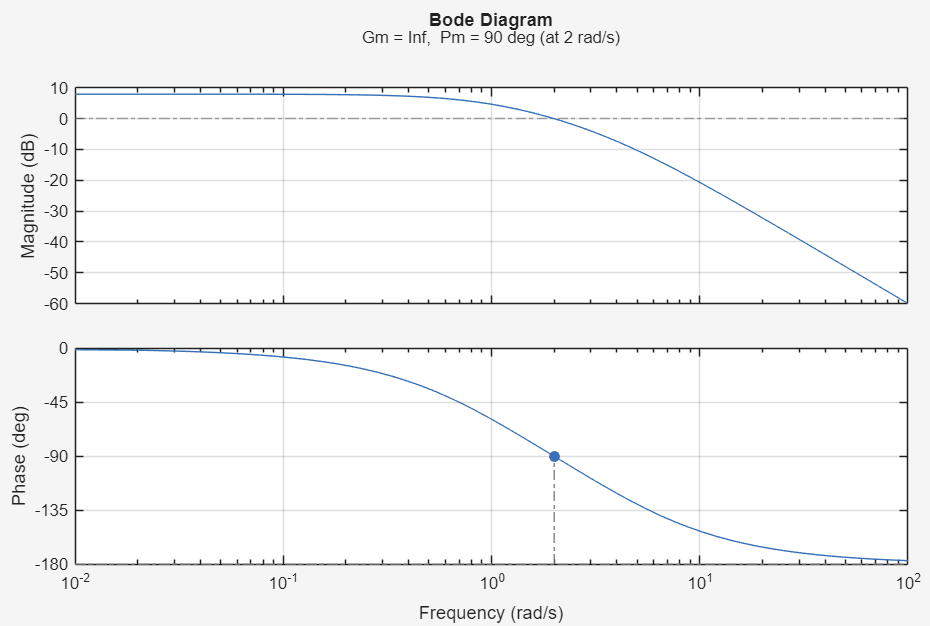
\includegraphics[width=0.7\textwidth]{P8-1.png}
\end{center}
The uncompensated system has a gain crossover frequency of $\omega_{gc}=2$ rad/s and a phase margin of 90 degrees.\\\\
\textit{I can add a lead compensator to maintain a decent phase margin while improving system response speed by increasing gain $K_c$. I will arbitrarily decide on a phase margin of 45 degrees.}
\begin{center}
    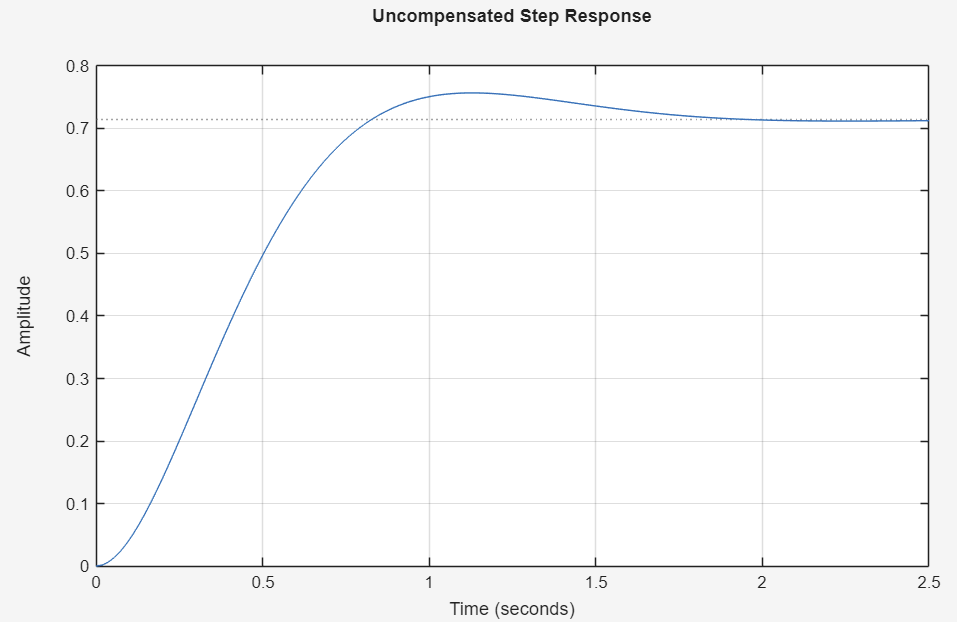
\includegraphics[width=0.7\textwidth]{P8-2.png}
\end{center}
From MATLAB, the step-response time specs are as follows:
\begin{lstlisting}
         RiseTime: 0.5435
    TransientTime: 1.6066
     SettlingTime: 1.6066
      SettlingMin: 0.6454
      SettlingMax: 0.7568
        Overshoot: 5.9523
       Undershoot: 0
             Peak: 0.7568
         PeakTime: 1.1237

Steady-state error: 0.2857
\end{lstlisting}
Since there is a steady-state error, I can add a lag compensator to reduce the steady-state error to a unit step input.
\begin{itemize}
    \item[1] \textbf{Determine lead compensator parameters:} I will choose an arbitrary lead compensator zero and pole location of $z=2$ and $p=8$, such that $z<p$.\\\\
    In MATLAB, I will iteratively increase the gain $K_c$ until the phase margin is 45 degrees, aiming for a higher crossover frequency of about double the uncompensated system's crossover frequency ($\omega_{gc,\text{ desired}} \approx 4$ rad/s).
    \begin{center}
        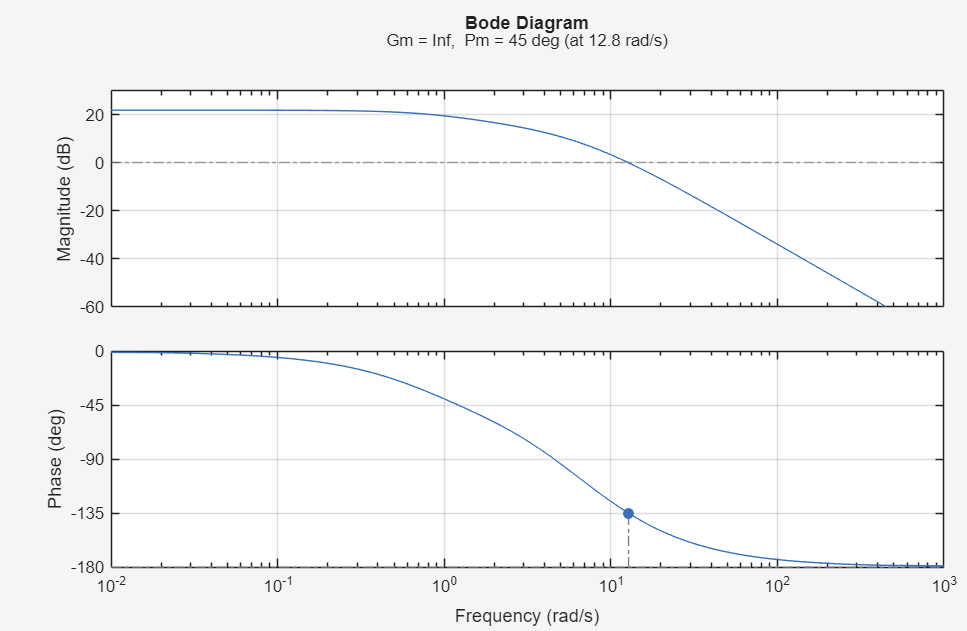
\includegraphics[width=0.7\textwidth]{P8-3.png}
    \end{center}
    For $K_c=20$, I found that
    \begin{lstlisting}
        Gain crossover: 12.78 rad/s
        Phase margin: 45.02 degrees
    \end{lstlisting}
    This is satisfactory, so I will keep the lead compensator parameters as $K_c=20$, $z=2$, and $p=8$.
    \item[2] \textbf{Determine lag compensator parameters:} Solving the steady-state error of the lead compensated system:
    \[
L(s)=\frac{20(s+2)}{s+8}\cdot\frac{10}{(s+1)(s+4)}=\frac{200(s+2)}{(s+8)(s+1)(s+4)}
\]
For a unit step input, the steady-state error is:
\[
\begin{aligned}
e_{ss}
&= \lim_{s\to 0}sE(s)\\
&= \lim_{s\to 0}s\cdot\frac{1}{s}\cdot\frac{1}{1+L(s)}\\
&= \lim_{s\to 0}
\frac{(s+8)(s+1)(s+4)}
{(s+8)(s+1)(s+4)+200(s+2)}\\
&= \frac{32}{32+400}\\
&= \boxed{\frac{2}{27}\approx 0.0741}.
\end{aligned}
\]
Thus, I will need to add a lag compensator to limit the steady-state error to a unit step input to be less than or equal to 0.01. Finding the ratio $z/p$ for the lag compensator:
\[C_{lag} = \frac{s+z}{s+p}\]
\[
\begin{aligned}
e_{ss}
&= \lim_{s\to 0}sE(s)\\
&= \lim_{s\to 0}s\cdot\frac{1}{s}\cdot\frac{1}{1+L(s)}\\
&= \lim_{s\to 0}
\frac{(s+8)(s+1)(s+4)(s-p)}
{(s+8)(s+1)(s+4)(s-p)+200(s+2)(s-z)}\\
&= \frac{-32p}{-32p+400z}\\
&= \frac{32p}{32p+400z}
\end{aligned}
\]
\[
\begin{aligned}
e_{ss} &= \frac{32p}{32p+400z}\leq 0.01\\
32p &\leq 0.32p+4z\\
31.68p &\leq 4z\\
\frac{z}{p} &\geq 7.92
\end{aligned}
\]
\end{itemize}
To keep the lag compensator's poles and zeros close to the origin, pick $p=0.1$ and $z=0.792$.
\textbf{Final Compensated Response}
\begin{center}
    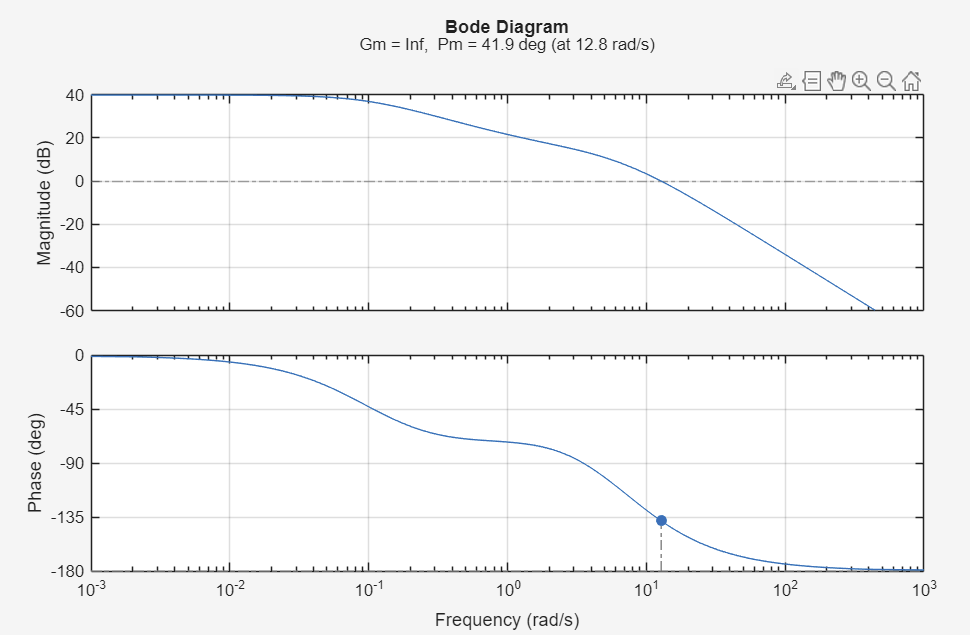
\includegraphics[width=0.9\textwidth]{P8 final.png}
\end{center}
\begin{center}
    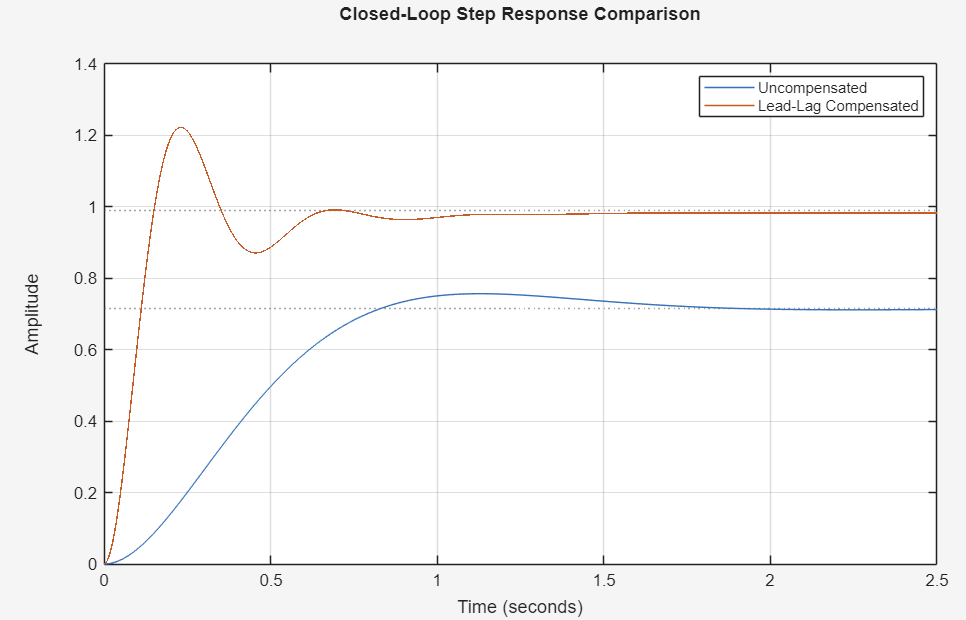
\includegraphics[width=0.9\textwidth]{P8 final-1.png}
\end{center}
Time specs:
\begin{lstlisting}
    Lead-Lag Compensated specs:
Gain crossover: 12.7911 rad/s
Phase margin: 41.88 degrees

ans = 

  struct with fields:

         RiseTime: 0.1013
    TransientTime: 1.0000
     SettlingTime: 1.0000
      SettlingMin: 0.8712
      SettlingMax: 1.2229
        Overshoot: 23.5227
       Undershoot: 0
             Peak: 1.2229
         PeakTime: 0.2299

Steady-state error: 0.0100
\end{lstlisting}
\end{document}
